\documentclass{beamer}
\mode<presentation>
\usepackage{amsmath}
\usepackage{amssymb}
%\usepackage{advdate}
\usepackage{adjustbox}
\usepackage{subcaption}
\usepackage{enumitem}
\usepackage{multicol}
\usepackage{mathtools}
\usepackage{listings}
\usepackage{url}
\def\UrlBreaks{\do\/\do-}
\usetheme{Boadilla}
\usecolortheme{lily}
\setbeamertemplate{footline}
{
  \leavevmode%
  \hbox{%
  \begin{beamercolorbox}[wd=\paperwidth,ht=2.25ex,dp=1ex,right]{author in head/foot}%
    \insertframumber{} / \inserttotalframenumber\hspace*{2ex}
  \end{beamercolorbox}}%
  \vskip0pt%
}
\setbeamertemplate{navigation symbols}{}

\providecommand{\nCr}[2]{\,^{#1}C_{#2}} % nCr
\providecommand{\nPr}[2]{\,^{#1}P_{#2}} % nPr
\providecommand{\mbf}{\mathbf}
\providecommand{\pr}[1]{\ensuremath{\Pr\left(#1\right)}}
\providecommand{\qfunc}[1]{\ensuremath{Q\left(#1\right)}}
\providecommand{\sbrak}[1]{\ensuremath{{}\left[#1\right]}}
\providecommand{\lsbrak}[1]{\ensuremath{{}\left[#1\right.}}
\providecommand{\rsbrak}[1]{\ensuremath{{}\left.#1\right]}}
\providecommand{\brak}[1]{\ensuremath{\left(#1\right)}}
\providecommand{\lbrak}[1]{\ensuremath{\left(#1\right.}}
\providecommand{\rbrak}[1]{\ensuremath{\left.#1\right)}}
\providecommand{\cbrak}[1]{\ensuremath{\left\{#1\right\}}}
\providecommand{\lcbrak}[1]{\ensuremath{\left\{#1\right.}}
\providecommand{\rcbrak}[1]{\ensuremath{\left.#1\right\}}}
\theoremstyle{remark}
\newtheorem{rem}{Remark}
\newcommand{\sgn}{\mathop{\mathrm{sgn}}}
\providecommand{\abs}[1]{\left\vert#1\right\vert}
\providecommand{\res}[1]{\Res\displaylimits_{#1}}
\providecommand{\norm}[1]{\lVert#1\rVert}
\providecommand{\mtx}[1]{\mathbf{#1}}
\providecommand{\mean}[1]{E\left[ #1 \right]}
\providecommand{\fourier}{\overset{\mathcal{F}}{ \rightleftharpoons}}
%\providecommand{\hilbert}{\overset{\mathcal{H}}{ \rightleftharpoons}}
\providecommand{\system}{\overset{\mathcal{H}}{ \longleftrightarrow}}
    %\newcommand{\solution}[2]{\textbf{Solution:}{#1}}
%\newcommand{\solution}{\noindent \textbf{Solution: }}
\providecommand{\dec}[2]{\ensuremath{\overset{#1}{\underset{#2}{\gtrless}}}}
\newcommand{\myvec}[1]{\ensuremath{\begin{pmatrix}#1\end{pmatrix}}}
\let\vec\mathbf

\lstset{
%language=C,
frame=single,
breaklines=true,
columns=fullflexible,
showstringspaces=false
}

\numberwithin{equation}{section}

\title{MATGEO Presentation: 2.10.82}
\author{S.Harsha Vardhan Reddy \\ ee25btech11054,\\IIT Hyderabad.}

\date{\today}
\begin{document}

\begin{frame}
\titlepage
\end{frame}

\section*{Outline}
\begin{frame}
\tableofcontents
\end{frame}

\section{Problem}
\begin{frame}[fragile]
\frametitle{Problem Statement}
Let $\vec{u}$, $\vec{v}$, and $\vec{w}$ be vectors in three-dimensional space, where $\vec{u}$ and $\vec{v}$ are unit vectors which are not perpendicular to each other and
$$ \vec{u}\cdot\vec{w} = 1, \quad \vec{v}\cdot\vec{w} = 1, \quad \vec{u}\cdot\vec{v} = 4. $$
If the volume of the parallelepiped, whose adjacent sides are represented by the vectors $\vec{u}$, $\vec{v}$, and $\vec{w}$, is $\sqrt{2}$, then the value of $|3\vec{u} + 5\vec{v}|$ is \_\_\_\_\_\_\_. (2021)
\end{frame}

\section{Solution}
\subsection{Calculation}
\begin{frame}{Calculation}
We are asked to find the magnitude of the vector $3\vec{u} + 5\vec{v}$. We will compute the square of its magnitude using the formula $||\vec{x}||^2 = \vec{x}^\top\vec{x}$.
\begin{align}
    ||3\vec{u} + 5\vec{v}||^2 &= (3\vec{u} + 5\vec{v})^\top (3\vec{u} + 5\vec{v}) \\
    &= 9(\vec{u}^\top\vec{u}) + 30(\vec{u}^\top\vec{v}) + 25(\vec{v}^\top\vec{v})
\end{align}
We are given that $\vec{u}$ and $\vec{v}$ are unit vectors, which means $\vec{u}^\top\vec{u} = 1$ and $\vec{v}^\top\vec{v} = 1$. We are also given the value $\vec{u}^\top\vec{v} = 4$.
\end{frame}

\begin{frame}{Final Result}
Substituting these values formally:
\begin{align}
    ||3\vec{u} + 5\vec{v}||^2 &= 9(1) + 30(4) + 25(1) \\
    &= 9 + 120 + 25 \nonumber \\
    &= 154
\end{align}
Taking the square root gives the magnitude:
\begin{equation}
    |3\vec{u} + 5\vec{v}| = \sqrt{154}
\end{equation}
\end{frame}

\subsection{Analysis}
\begin{frame}{Note on the Problem Statement}
There appears to be a contradiction in the problem statement. 
\vspace{1em}

The vectors $\vec{u}$ and $\vec{v}$ are given as \textbf{unit vectors}. The dot product of two unit vectors is defined as:
$$ \vec{u} \cdot \vec{v} = ||\vec{u}|| \cdot ||\vec{v}|| \cos\theta = (1)(1)\cos\theta = \cos\theta $$
Since the value of $\cos\theta$ must be in the range $[-1, 1]$, the given value $\vec{u}\cdot\vec{v} = 4$ is impossible.
\end{frame}

\section{Plot}
\begin{frame}{Plot}
 \begin{figure}[H]
     \centering
     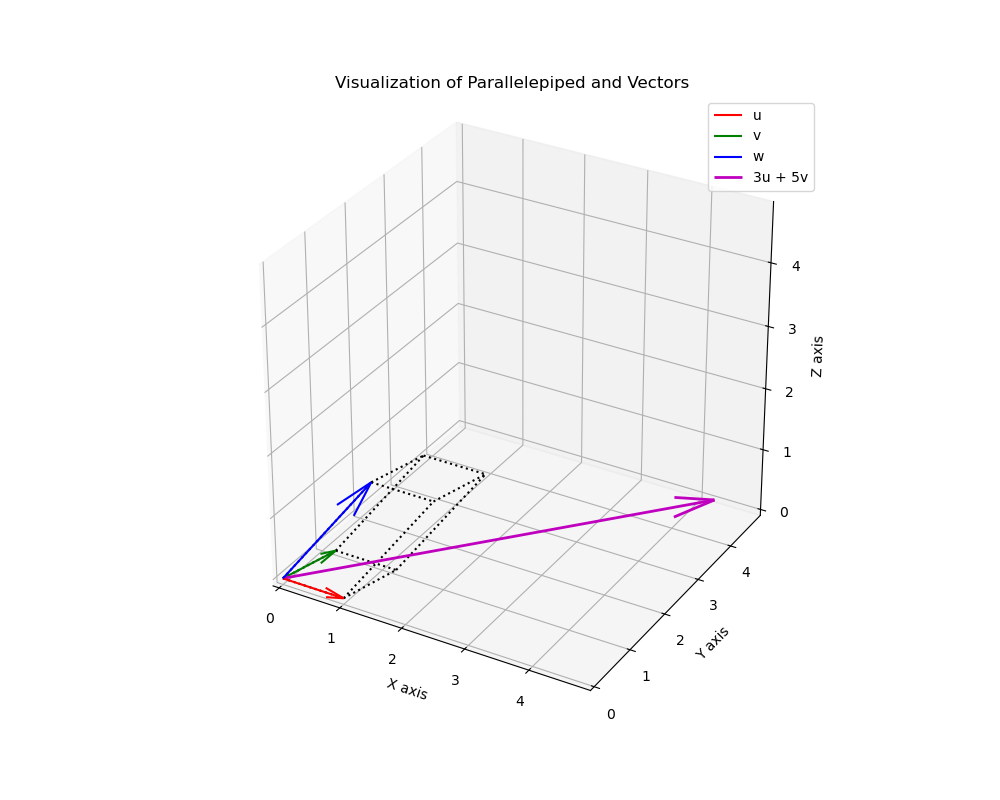
\includegraphics[width=\columnwidth]{../figs/2.10.82 2 .png}
     \caption*{}
     \label{fig:plot_placeholder}
 \end{figure}
\end{frame}

\end{document}